% ---
% asset_id: FA22TravellingSalesmanProblemTikZ-001
% asset_type: tikz
% topic_id: FA22TravellingSalesmanProblem
% unit_code: FA22
% topic_code: FA22-ALGGRAPH
% lesson_file: FA22_travelling_salesman_problem_lesson.md
% related_lesson_section: "# 9. Visual Asset Integration"
% used_placeholder: "[VISUAL PLACEHOLDER: FA22TravellingSalesmanProblemTikZ-001 | Source: AI-proposed teaching enhancement based on uploaded NNA evidence | Insert from tikz/FA22TravellingSalesmanProblemTikZ-001.tex | Purpose: Provide a clean weighted complete graph matching the main generated nearest-neighbour worked example.]"
% ---

\documentclass[tikz,border=8pt]{standalone}
\usepackage{tikz}
\usetikzlibrary{arrows.meta,positioning,calc}
\begin{document}
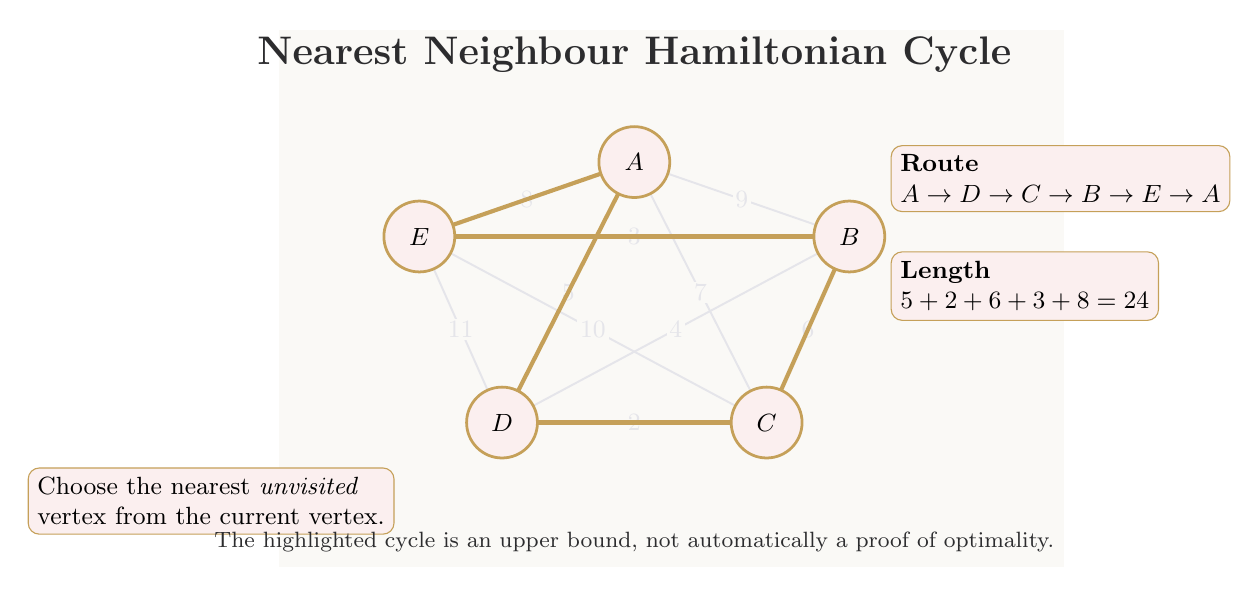
\begin{tikzpicture}[scale=1.05, every node/.style={font=\small}]
\definecolor{CANVAS}{HTML}{FAF9F6}
\definecolor{DIVIDER}{HTML}{E5E5EA}
\definecolor{GOLD}{HTML}{C5A059}
\definecolor{PINKFILL}{HTML}{FBEFEF}
\definecolor{TEXTCOL}{HTML}{2C2C2E}
\fill[CANVAS] (-4.3,-3.3) rectangle (5.2,3.2);
\node[font=\Large\bfseries,text=TEXTCOL] at (0,2.9) {Nearest Neighbour Hamiltonian Cycle};
\coordinate (A) at (0,1.6);
\coordinate (B) at (2.6,0.7);
\coordinate (C) at (1.6,-1.55);
\coordinate (D) at (-1.6,-1.55);
\coordinate (E) at (-2.6,0.7);
\foreach \p/\q/\w in {A/B/9,A/C/7,A/D/5,A/E/8,B/C/6,B/D/4,B/E/3,C/D/2,C/E/10,D/E/11}{\draw[DIVIDER,line width=.7pt] (\p)--(\q) node[midway,fill=CANVAS,inner sep=1pt] {\(\w\)};}
\draw[GOLD,line width=1.5pt,-{Latex[length=2.5mm]}] (A)--(D);
\draw[GOLD,line width=1.5pt,-{Latex[length=2.5mm]}] (D)--(C);
\draw[GOLD,line width=1.5pt,-{Latex[length=2.5mm]}] (C)--(B);
\draw[GOLD,line width=1.5pt,-{Latex[length=2.5mm]}] (B)--(E);
\draw[GOLD,line width=1.5pt,-{Latex[length=2.5mm]}] (E)--(A);
\foreach \p in {A,B,C,D,E}{\node[circle,draw=GOLD,fill=PINKFILL,line width=1pt,minimum size=9mm] at (\p) {\(\p\)};}
\node[draw=GOLD,fill=PINKFILL,rounded corners,align=left,anchor=west] at (3.1,1.4) {\textbf{Route}\\ \(A\to D\to C\to B\to E\to A\)};
\node[draw=GOLD,fill=PINKFILL,rounded corners,align=left,anchor=west] at (3.1,0.1) {\textbf{Length}\\ \(5+2+6+3+8=24\)};
\node[draw=GOLD,fill=PINKFILL,rounded corners,align=left,anchor=east] at (-2.9,-2.5) {Choose the nearest \emph{unvisited}\\vertex from the current vertex.};
\node[font=\footnotesize,text=TEXTCOL] at (0,-3.0) {The highlighted cycle is an upper bound, not automatically a proof of optimality.};
\end{tikzpicture}
\end{document}
